\documentclass[12pt]{article}
\usepackage{geometry}
%\geometry{left = 3cm, right = 2.5cm, top = 2.5cm, bottom = 2.5cm}
\usepackage{graphicx}
\usepackage{cite}
\title{Improved genetic algorithm for finding shortest paths problem}
\author{Qi Yixi}
\date{\today}
\begin{document}
%\huge
\maketitle{}
\section{Introduction}
%\subparagraph{
	The optimal path problem is a very classical mathematical problem, which is the basis for many optimization problems such as resource allocation, path analysis and design. The shortest path algorithm can be divided into a single vertex shortest path algorithm, and a shortest path algorithm between each pair of vertices. A typical solution to converntional route planning problems is the Dijkstra algorithm, which has used in road networks and in dynamic environments to find a route minimizing the travel time from an origin to a destination. However in the practical application, the size of the shortest path problem is expanding, the constraint condition of the shortest path problem is increasing. In the traditional algorithm, it is difficult to effectively find a perfect solution to quickly find the optimal solution or suboptimal solution, and then some study use the genetic algorithm to find the shortest path.
\subsection{Genetic algorithm}
Genetic algorithm is a computational model simulating the natural selection and genetic mechanism of Darwinian biological evolution, and it is a method to search the optimal solution by simulating the natural evolution. Genetic algorithm starts from a population which represents the potential solution set of the problem, and a population is composed of a certain number of individuals encoded by gene. The steps of the Genetic algorithm are firstly generation some population. After the generats of the first generation of population, according to the survival of the fittest , generation evolves generation by generation to produce better and better approximate solutions. In each generation, individuals are selected according to the fitness of individuals in the problem domain, and with the help of nature. Genetic operators in genetics carry out cross and mutation to produce populations representing new solution sets. This process will result in the population of the posterity, like the natural evolution, more adaptable to the environment than that of the previous generation. The optimal individuals in the last generation can be decoded as the approximate optimal solution of the problem. Genetic algorithm generates many solutions to a single problem each one with different performance some are better than other in performance. So it have been successfully applied to many aspects, like optimization, and machine learning problems. The evolutionary process consists of maintaining a population of coded solutions which are manipulated by variation operators to find a satisfactory optimized solution. Such as find the optimal path, the writer used GA to help the robot path planning\cite{Alnasser2016}, and then they find the GA is more efficiency and effectiveness. 
Many studies using genetic algorithm to solve multi-objective route planning problems have been reported\cite{Diao2019}, which include a review of recent issue and applications to mobile robots, personal navigation, tourist sight sight-seeing itinerary and personal navigation. In the other hands, the JunWoo\cite{Kim2019} kim studies the candidate order based genetic algorithm to solve the maze-type shortest path problem, and then the author compared Fitness Switching Genetic Algorithm and Candidate Order based Genetic Algorithm.
\subsection{pruning algorithm}
Pruning algorithm used in many aspects, such as in the machine learning and the decision tree. During the operation of the decsion tree, a large number of detail and complex trees will be generated. Just as genetic algorithm in this study generates a large number of offspring, each attribute(offspring) must be considered in detail. Not only for the considering tree, but also for the genetic algorithm, a large number of data can guarantee high accuray, but too much data also brings about redundant computation.  In the decision tree algorithm, the algorithm has two kind of pruning plain, one is preprune, and the other is the post-pruning. Pre-prune means prune  by stopping the structure of the tree in advance, and the post-pruning means prune after the tree genegrates a large number of suntree.
\section{Research purposes}
%\subparagraph{
Traditional genetic algorithm always used in the machine learning, in the past years, people find it can use in the find path problem, With the graph nodes grow, the genetic algorithm has the less time cost than the dijkustra algorithm. However, in order to get the best answer, the traditional genetic algorithm needs to generate a large number of random offsprings to find the optimal rout, with the graph nodes increase, the computing consumption increase,too. Because of the crossover step can not generate the right path at once, the genetic aglorithm have to generate more offspring to find the right one. From the study, we know that the crossover operator in genetic algorithm controls the generation of offspring. At present, some study give us different crossover operator, but they did not to use them in the find shortest path. So in this paper, we will use these different crossover operator to reduce the offspring number and then use the pruning algorithm to prun the useless offspring. less offspring means save time and the storage space.

\section{Related research}	
%\subsection{Genetic algorithm}
%\subparagraph{
Techniques like Dijkstra, Floy-warshall and Bellman ford are the most commonly used algorithms for evaluating shortest paths. especially the Dijkstra, not only in the static environment, but also in the dynamic environment\cite{10.1007/978-3-319-60042-0_15}, the Dijkstra was the most popular algorithms in the past years. Whith the time goes by, the amount of data that needs to be processed is also increaing, compared to the Dijkstra algorithm, the genetic algorithm have the better resulty to solve the big data shortest path problem\cite{Wang2018}. So some studies have begun to focus on solving the shortest path  problem with genetic algorithm. In the recently, one research using GAs to solve the supermarket manger traveling problem\cite{Al-hayali2018}.This is one of the shortest path problem,the writer makes a GAs models and then use an example to show the GAs is an efficient method to provide optimizations of these problems.But this study just use the genetic algorithm to sovle the best path problme, and it have to process a large amount of the population datas. So, Some study impoved the genetic algorithm and use improved GAs to solve the multi-objective route planning problems in dynamic environment\cite{Kanoh2008}. He gives one new crossover operator and compared with traditional GAs and Dijkstra algorithm, the improved GAs cost a less time than DA and raditional GAs. So we think change the different crossover can improved the genetic algorithm. Puljic and Manger \cite{Puljic2013} worked upon comparison of eight evolutionary crossover operators for the vehicle routing problem. The eight evolutionary crossover operators are order crossover, partially mapped crossover, edge recombination crossover, cycle crossover, alternating edges crossover, heuristic greedy crossovers, random crossover and probabilistic crossover. They restricted themselves to investigate relative strengths and weaknesses of various crossover operators and claimed that the results obtained will help in construction of sophisticated algorithms in future. Chand and Mohanty \cite{Chand2013} considered a multi-objective vehicle routing problem using dominant rank method with the objectives of minimizing the number of vehicles and total cost (distance). They used Sub Route Mapped Crossover Method (SMCM) and Sub Route Exchange Mutation Method (SEMM) as genetic operators. They applied dominant rank method to get Pareto optimal set and they claimed that their method finds optimum solutions effectively. In the past year, A.J. Umbarkar and P.D. Sheth\cite{Umbarkar2015} sums up crossover operator, some of them fit the binary coding problem, some of them fit the real number coding problem. but they only introduce the different crossover operator, not to use or compare them.  


However, regardless of the purpose of their use of the genetic algorithm it is inevitable that one problem is that the data volume of the genetic algorithm is too large, because the genetic algorithm generates a large amount of offspring data. So in this paper, we will try to use pruning algorithm to reduce the time cost.

%%%%%%% 
The shortest path problems always a Genetic algorithm starts from a population which represents the potential solution set of the problem, and a population is composed of a certain number of individuals encoded by gene. 
%\subsection{The pruning algorithm}
 



\section{Research plan}
%\subparagraph{
Implementation Genetic algorithm, which following step is in the figure1
1. Implementation the genetic algorithm as fllow steps:
\subsection{Coding and decoding}
%\subparagraph{
Coding the all of the graph point. Randomly generate sequences to form the original chromosome as the initial population, the length is the total number of points in the graph. Then use the depth traversal algorithm to get the decoding shortest path based on the node id.
\subsection{Set the fitness function}
%\subparagraph{
The fitness function is an important section in the genetic algorithm. From the table 1, the fitness function needs to calculate the individual fitness value, and then judgment the direction of evolution. Use fitness function can choose the best individual and then choses the generate direction. From the recently study\cite{Gunturu2017}, the reasercher use the fitness function to find game equilibria, the result proposed  fitness function increase the efficiency of Genetic Algorithms. 
\subsection{Crossover operator }
%\subparagraph{
Crossover operator used to combine the genetic information of two parents to generate new offspring. It is a one way to stochastically generate new solutions from an existing population. this is one of important process in the Genetic algorithm. This is one of important part in this paper, we will use five different crossover operator to find the optimal path.

1.Partial-Mapped Crossover (PMX)
Randomly select the starting and ending positions of several genes in a pair of chromosomes (the two chromosomes are selected at the same position), and then exchange the positions of these two groups of genes:

For conflict detection, establish a mapping relationship according to the two groups of exchanged genes, as shown in the figure. Take the mapping relationship of figure2 as an example, it can be seen that the second step results that there are two genes 1 in sub generation 1, and then transform them into gene 3 through mapping relationship, and so on until there is no rush. Finally, all the conflicting genes will be mapped to ensure that the new pair of offspring genes will not conflict.

2.Order Crossover (OX)
As same with PMX, the starting and ending positions of several genes in a pair of chromosomes (parents) were randomly selected (two chromosomes were selected at the same positions), generation of a offspring, and ensure that the location of the selected gene in the offspring is the same as that of the parent,
and then find out the position of the gene selected in the first step in another parent, and then put the remaining genes into the offspring generated in the previous step in order.


3.Position-based Crossover (PBX)
Several genes in a pair of chromosomes (parents) were randomly selected, but the positions of the two chromosomes were the same. In the same way as the second step of ox, a offspring is generated and the position of the selected gene in the offspring is the same as that of the parent. It is also the same as the third step of ox, first find out the location of the selected gene in the first step in another parent, and then put the remaining genes into the offspring generated in the previous step in order.




4.Order-Based Crossover (OBX)
Several genes in a pair of chromosomes (parents) were randomly selected, but the positions of the two chromosomes were the same,find the location of the selected gene of the parent 1 in the parent 2, and then generate the offspring with the rest of the genes in the parent 2, and ensure the location correspondence, and put the selected genes from the parent 1 into the remaining positions of the offspring in order:



5.Subtour Exchange Crossover
Select a group of genes on one parent and find the positions of these genes on the other parent:
Keeping the unselected genes unchanged, according to the sequence of the selected genes, exchange the positions of genes in the chromosomes of the two parents, and generate two offspring at a time:


\subsection{Mutation operator}
%\subparagraph{
The mutation operator is an auxiliary method, and it has an effect on the local search ability of genetic algorithm. Mutation operator can change the individual chromosome to make a new chromosome, it can help the algorithm get some new solution and then avoid the local optimum.
\subsection{Add Pruning algorithm}
%\subparagraph{
 After crossover operator and mutation operator, traditional genetic algorithm will use the fitness function to judgement the offspring, if the offspring fit the fitness function, then it will be the end result. In general, after crossover operator and mutation operator, we will get a lot of offspring However some offspring graduated by random crossover operated, so they are useless.If these offspring enter the fitnessfuction, It must cost more computer time and occupy storage space. So in this paper will use the post-pruning to pruning the useless offspring. 
\subsection{Compare with the traditional genetic algorithm }
%\subparagraph{
To proposed the improved Genetic algorithm's advantage, after implementation the genetic algorithm, this paper will compared the different algorithm and then use the data to test the algorithm. 

	\small
	\bibliographystyle{plain}
	\bibliography{1}
%picture
\begin{figure}[h]
	\centering
	\includegraphics{f11}
	\caption{Fig. 1. PMX}
\end{figure}

\begin{figure}[h]
	\centering
	\includegraphics{f12}
	\caption{Fig. 2. PMX}
\end{figure}

\begin{figure}[h]
	\centering
	\includegraphics{f2}
	\caption{Fig. 3. OX}
\end{figure}

\begin{figure}[h]
	\centering
	\includegraphics{f3}
	\caption{Fig. 4. PBX}
\end{figure}

\begin{figure}[h]
	\centering
	\includegraphics{f4}
	\caption{Fig. 5. OBX}
\end{figure}

\begin{figure}[h]
	\centering
	\includegraphics{f5}
	\caption{Fig. 6. Subtour Exchange Crossover}
\end{figure}


\begin{figure}[h]
	\centering
	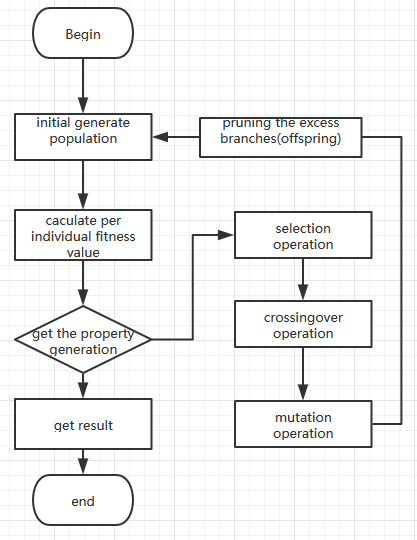
\includegraphics{flowchart1}
	\caption{flowchart}
\end{figure}


%\cite{1}
%\begin{thebibliography}
%\bibliographystyle{plain}
%\bibliography{1}
%\end{thebibliography}
\end{document}
